% -*- mode: fundamental -*-

% ****************************************************************

\chapter{Introduction}

\markboth{Ch \arabic{chapter}: Introduction (DRAFT)}{\copyrightnotice}


\setcounter{page}{1}
% \renewcommand{\thepage}{\arabic{page}}
\renewcommand{\thepage}{\arabic{chapter}-\arabic{page}}

\label{ch_intro}

% ****************************************************************

``Digital Design'' and ``CPU Design'' (or ``Computer Architecture'')
are traditionally taught separately, usually in that order, with
separate textbooks.  Digital Design is usually taught using one of the
traditional hardware design languages Verilog, SystemVerilog or VHDL,
and often makes use of small, often artificial examples.  CPU Design
is often taught without actually designing hardware, relying instead
on textbooks, abstract schematics, and simulators implemented in
software.

This book takes a different approach: we learn about simple CPU
architectures by designing them with a modern Hardware Design Language
(HDL) called BSV, learning Digital Design as an ongoing, intertwined
accompanying topic.  Each Digital Design example will be taken
directly from the CPU Design, so that the example's use-case (context)
is always perfectly clear, and the reader always has a clear sense of
the purpose of the example.

The CPU we design here will execute instructions from the RISC-V
Instruction Set Architecture (ISA), which is an industrial-strength
ISA (with many commerical implementations).  Our designs will be
simple (typical of small, embedded systems and micro-controllers, not
laptops/workstations or servers).  Nevertheless, it will be powerful
enough to execute Linux, an industrial-strength operating system.

Figure~\ref{fig_Topics} shows the plan for topics covered in this book.
\begin{figure}[htbp]
  \centerline{\includegraphics[width=6in,angle=0]{ch010_intro/Figures/fig_Topics}}
  \caption{\label{fig_Topics}Topics covered (in red text in red box)}
\end{figure}

\begin{itemize}

\item The first step is to understand the RISC-V ISA itself.  What are
    RISC-V instructions, how are they coded in bits, and what do they
    mean?  This topic is not a focus of this book (for which there are
    plenty of textbooks available), but understanding the ISA is of
    course a prerequisite to informing our design.  The RISC-V ISA has
    many options; our focus will be on a ``standard'' suite:

    \begin{tightlist}
		  
      \item From the RISC-V Unprivileged ISA spec: basic integer
        arithmetic and logic operations; branch and jump; load and
        store; integer multiply and divide; atomic memory operations;
        floating-point operations; compressed instructions (so-called
        RV32IMAFDC and RV64IMAFDC).

      \item From the RISC-V Privileged ISA spec: handling traps and
        interrupts; Control and Status Registers (CSRs); Machine,
        Supervisor and User Privilege levels.

    \end{tightlist}


\item In order to run actual RISC-V programs on our implementations,
    we need to undertand how to use the \emph{riscv-gcc} compiler to
    compile C and RISC-V Assembly Language programs into RISC-V
    binaries (so-called ``ELF'' files).  Another useful tool is
    \emph{riscv-objdump}, which can disassemble the binary back into
    assembly-language text. This is useful for debugging our
    implementation, so that we can understand execution
    instruction-by-instruction, and diagnose anything that goes wrong.

    So, far, all this is not implementation-specific, {\ie} it is
    generic information about RISC-V.

\item A RISC-V CPU and system can be \emph{modeled} in a simulator
    coded in C (say).  Such a C-based simulator is compiled (with
    \emph{gcc}, say) and run like any other C program. We will not be
    discussing this much in this book.

\item We will code our hardware design in the BSV HDL.  We will use
    BSV not just for the CPU itself, but also for the ``system''
    components around it: an interconnect, Memory, UART and GPIO.
    Later we will discuss MMUs (Memory Management Units) and Caches,
    and possibly other devices and accelerators.

\item We will learn how to use the \emph{bsc} compiler to translate
    our BSV code into Verilog RTL.

\item We will learn how our Verilog RTL can directly be simulated in a
    Verilog simulator.  We will use the free, open-source
    ``Verilator'' simulator, but you can also run it on any other
    Verilog simulator, available from a number of providers.

    This will provide an exact, cycle-by-cycle accurate simulation of
    the very same design that we'll run later on an FPGA.  This is
    invaluable for debugging the hardware design, because the
    turnaround time to fix a problem and run a new simulation is very
    short (minutes) compared to creating a new version for an FPGA
    (several hours).

    Of course, Verilog simulation will run much more slowly (10,000x
    or more slower) compared to an FPGA, and so is useful primarily
    for early debugging and analysis of the design, running on small
    RISC-V programs.

\item When we execute our Verilog RTL hardware design in Verilog
    simulation (where the hardware design itself is executing a RISC-V
    binary program), it will produce a trace file describing events
    during the simulation.  We will learn how to analyze these traces
    to identify bugs and bottlenecks in our design, from which we can
    correct design errors and possibly improve performance.

\item We will learn now to process our Verilog RTL through an FPGA
    synthesis tool to create an FPGA bitfile which can then be loaded
    into an FPGA and executed.

    Although it can be synthesized and run on a number of FPGAs from
    different vendors, in this book we'll discuss how to build and run
    it for an FPGA on the Amazon AWS cloud.

\item Our Verilog RTL can also be processed through ASIC synthesis
    tools targeting ASIC fabrication.  We will not be dicsussing this
    much in this book.

\end{itemize}

We will create two hardware designs.  The first design is
``Magritte'', a \emph{non-pipelined} implementation\footnote{ See
Ren\'e Magritte, Belgian surrealist painter and his famous piece
labeled \emph{``Ceci n'est pas une pipe''} (``This is not a pipe'')
\url{https://en.wikipedia.org/wiki/Rene_Magritte}} which will
familiarize us all the basic concepts and flows (the RISC-V ISA,
preparing and running a RISC-V binary to run on the design, analysing
traces), without being distracted by the complexities of pipelineing
for high performance.  The second design is ``Fife'', which has a
five-to-six stage, mostly in-order pipeline, which is a
microarchitectural change focused on higher performance (speed) than
Magritte.  Both will execute exactly the same binaries; the only
difference will be in Fife's superior performance (speed).  Both
designs will share a large part of the BSV code implementing the
essential functionality for executing the RISC-V ISA.

As we work through the two designs, we will concurrently learn how to
code in BSV, the HDL for our designs.  BSV is a modern, high-level HDL
taking inspiration from modern software programming languages, in
particular the Haskell functional programming language and a class of
formal specification languages for concurrent programming (including
Term Rewriting Systems, Unity, TLA+, and Event-B).  BSV is not just
for CPU design; like Verilog and SystemVerilog, it is a ``universal''
language for any digital design, whether related to CPUs or not.

Please see Appendix~\ref{apx_resources} for a detailed listing of
resources (documents and software tools) needed for this book.

% ****************************************************************
